\section{Single Qubit Operations}
Any operation on a single qubit is an invertible function $f:|\psi\rangle \rightarrow |\psi \rangle$. In matrix form , it can be written as a $2 \times 2$ Unitary matrix $U$. The criteria that the matrix must be unitary arises from the fact that operations must be reversible and it must preserve the inner product. The following table mentions the most common quantum gates along with their matrix representations.
\begin{figure}[h]
\centering
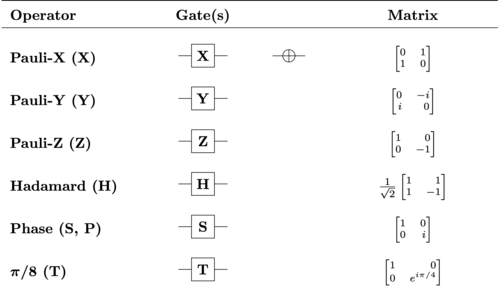
\includegraphics[width=0.95\textwidth]{images/singlegates.png}\par
\label{singlegates}
\caption{Common single qubit gates}
\end{figure}
\\The first three gates($X,Y,Z$) are the Pauli spin matrices signifying a rotation of $\pi$ in the bloch sphere notation along the respective axes.\\
The rotations by an angle $\theta$ along the $\hat{x}$, ,$\hat{y}$ and $\hat{z}$ axes are given by:
\begin{equation}
R_x(\theta) = e^{-i\theta X/2} = \cos{\frac{\theta}{2}}I - i\sin{\frac{\theta}{2}}X = \left[ {\begin{array}{cc}
   \cos{\frac{\theta}{2}} & -i\sin{\frac{\theta}{2}} \\
   -i\sin{\frac{\theta}{2}} & \cos{\frac{\theta}{2}} \\
  \end{array} } \right]
\end{equation}
\begin{equation}
R_y(\theta) = e^{-i\theta Y/2} = \cos{\frac{\theta}{2}}I - i\sin{\frac{\theta}{2}}Y = \left[ {\begin{array}{cc}
   \cos{\frac{\theta}{2}} & -\sin{\frac{\theta}{2}} \\
   \sin{\frac{\theta}{2}} & \cos{\frac{\theta}{2}} \\
  \end{array} } \right]
\end{equation}
\begin{equation}
R_z(\theta) = e^{-i\theta Z/2} = \cos{\frac{\theta}{2}}I - i\sin{\frac{\theta}{2}}Z = \left[ {\begin{array}{cc}
   e^{-i\theta/2} & 0\\
   0 & e^{i\theta/2}  \\
  \end{array} } \right]
\end{equation}
Since, every operator can be considered as a rotation in the Bloch sphere notation, there will exist some $\hat{n}$ and $\theta$ for all operators $U$ such that $U$ can be seen as a rotation of angle $\theta$ about $\hat{n}$ axis. 
\begin{equation}
U=R_n(\theta) = e^{-i\theta \hat{n}\cdot \overline{\sigma}/2} = \cos{\frac{\theta}{2}}I - i\sin{\frac{\theta}{2}}(n_x X + n_y Y + n_z  Z) 
\end{equation}
($\overline{\sigma} = X\hat{x} + Y\hat{y} + Z\hat{z}$ is often known as spin matrix vector. )\\
An important theorem is the $Z-Y$ decomposition of single qubit gates. It says that any unitary operator $U$ can be written in the form
\begin{equation}
U= e^{i\alpha} R_z(\beta)R_y(\gamma)R_z(\delta)
\end{equation}
where $\alpha, \beta, \gamma,  \delta$ are some real numbers. An intuitive way to think about this is that we first rotate the axes such that the y-axis aligns with $\hat{n}$, then perform the rotation and then bring the y-axis back to the correct position by reverse operations. More formally, any unitary operator can be written in the form
\begin{equation}
U = \left[ {\begin{array}{cc}
   e^{i(\alpha -\beta/2-\delta/2)} \cos{\frac{\gamma}{2}} & -e^{i(\alpha -\beta/2+\delta/2)} \sin{\frac{\gamma}{2}}\\
   e^{i(\alpha +\beta/2-\delta/2)} \sin{\frac{\gamma}{2}} & e^{i(\alpha +\beta/2+\delta/2)} \cos{\frac{\gamma}{2}}  \\
  \end{array} } \right]
\end{equation}and hence the form arises arises from simple matrix multiplication. In fact, we may replace $\hat{z}$ and $\hat{y}$ by any other non-collinear unit vectors. Another useful form in which the operator can be expressed is 
\begin{equation}
U = e^{i\alpha}AXBXC \text{ where A,B and C are matrices such that } ABC = I
\end{equation}In terms of the previous representation, we can deduce A,B and C as:
\begin{equation}
\begin{split}
A & = R_z(\beta)R_y(\frac{\gamma}{2})\\
B & = R_y(-\frac{\gamma}{2})R_z(-\frac{\delta+\beta}{2})\\
C & =R_z(\frac{\delta-\beta}{2})
\end{split}
\end{equation}\section{Controlled Operation}
The Controlled operations are used to do conditional operations. It takes two qubits, one control qubit and another target qubit, and performs a given operation $U$ on the target qubit if the control qubit is set to $|1\rangle$. \\
The most famous Controlled operation is the Controlled-NOT({\scshape CNOT}). It performs the not operation on the target qubit if the control qubit is set. Another way to represent it is  {\scshape CNOT}: $|c\rangle |t\rangle \rightarrow |c\rangle|c \oplus t\rangle$. 
\newpage
\begin{figure}[t]
\centering
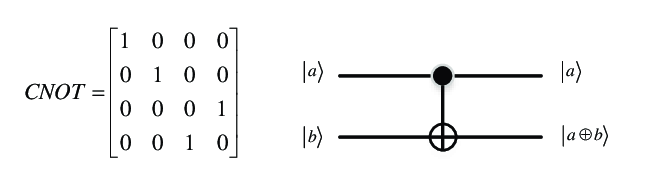
\includegraphics[width=0.5\textwidth]{images/cnot.png}\par
\label{cnot}
\caption{Representation and matrix associated with C-NOT gate}
\end{figure}
Any other controlled operator can be expressed with the help of {\scshape CNOT} gate and single qubit gates using the representation mentioned in Equation 3.10 . The circuit for Controlled-$U$ gate is shown below:
\begin{figure}[h]
\centering
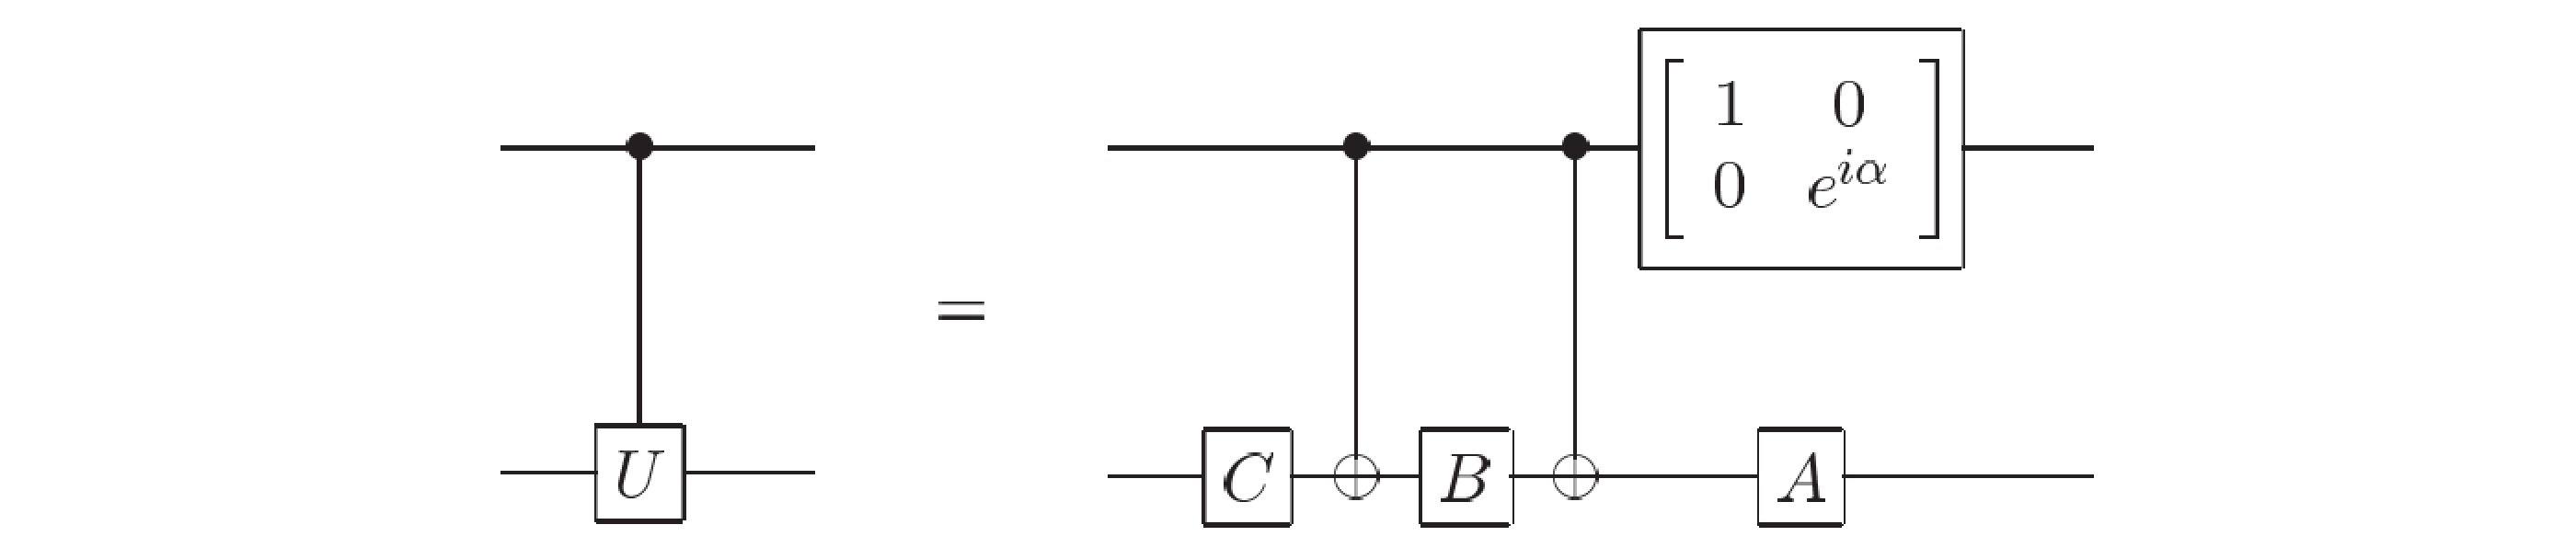
\includegraphics[width=1\textwidth]{images/cu.png}\par
\label{cU}
\caption{Circuit for Controlled- U gate where U =$e^{i\alpha}AXBXC$}
\end{figure}
\newline
The circuit can easily be verified to the controlled operator corresponding to the operator $U$. When the control qubit(the top one) is set to $|0\rangle$, then no change occurs as $ABC = I$ .  On the other hand, when the control qubit is $|1\rangle$ then operator $U = e^{i\alpha} AXBXC$ acts on the second qubit(the bottom one).\\
The controlled operator can be extended to have multiple control and target qubits. Such an operator applies $U$ on the target qubit(s) if all the control qubits are $|1\rangle$. We use the following representation where $|x_1\rangle,|x_2\rangle...|x_n\rangle$ are n control qubits and $|\psi\rangle$ is the composite state of the target qubits.
\begin{equation}
C^n(U)|x_1,x_2...x_n\rangle|\psi \rangle = |x_1,x_2....x_n\rangle U^{x_1x_2.....x_n}|\psi\rangle
\end{equation}Any $C^2(U)$ can be implemented as the following circuit if $U = V^2$ for some unitary matrix $V$. 
\begin{figure}[h]
\centering
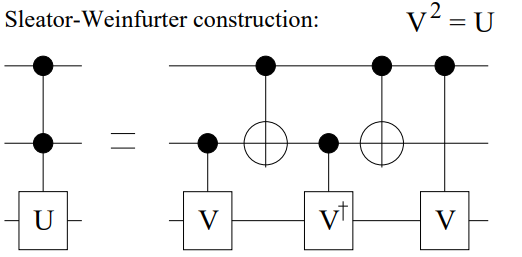
\includegraphics[width=0.93\textwidth]{images/c2.png}\par
\label{cU}
\caption{Circuit for $C^2(U)$ gate where $U = V^2$}
\end{figure}
\newline
The famous Toffoli gate is $C^2(X)$ and can be implemented as follows:
\begin{figure}[h]
\centering
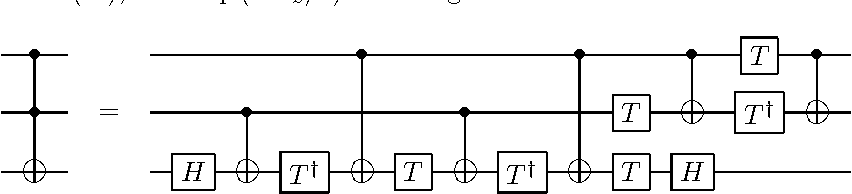
\includegraphics[width=0.93\textwidth]{images/toffoli.png}\par
\label{toffoli}
\caption{Circuit for $C^2(X)$ i.e. Toffoli gate }
\end{figure}
\newline
{\centering (Here we have to use both the reductions in the section i.e. $C^2$ from $C^1$ and $C^1$ from {\scshape CNOT} )}\\
For general $C^n(U)$ gate we will have to use some extra qubits known as ancilla bits. The following circuit shows how to implement $C^n(U)$:
\begin{figure}[h]
\centering
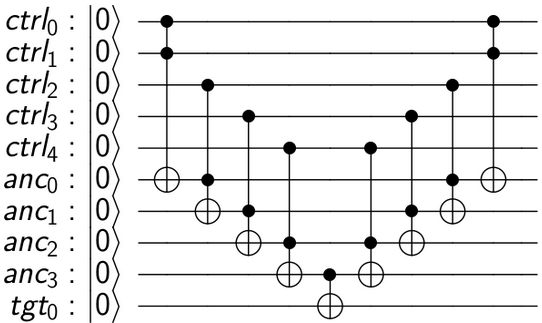
\includegraphics[width=0.5\textwidth]{images/cn.png}\par
\label{cn}
\caption{Circuit for $C^n(U)$ gate. Here n=5}
\end{figure}
\newline
It turns out that any $C^n(U)$ gate can be implemented using $O(n^2)$ Toffoli, {\scshape CNOT}, and single qubit gates.
(\href{https://algassert.com/circuits/2015/06/05/Constructing-Large-Controlled-Nots.html}{This guy} even reduced it to $O(n)$ for $U=X$).